%%%%%
\begin{figure}[!ht]
\centering
  \hfill\subfloat[ii=24]{
  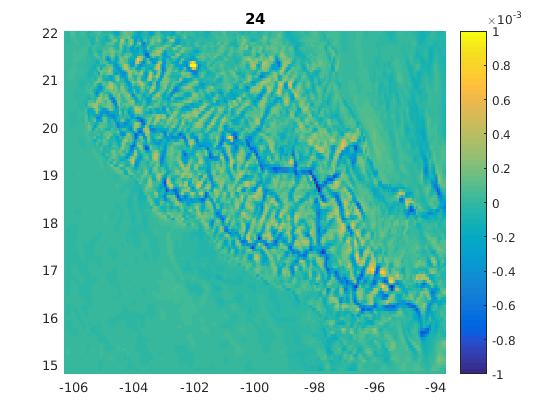
\includegraphics[width=0.35\textwidth]{div1}
  }\hfill
  \subfloat[ii=29]{%\label{fig:}
  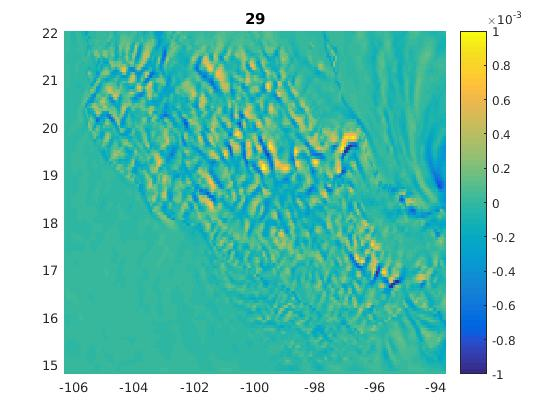
\includegraphics[width=0.35\textwidth]{div2}
  }\hfill

  \hfill\subfloat[ii=34]{
  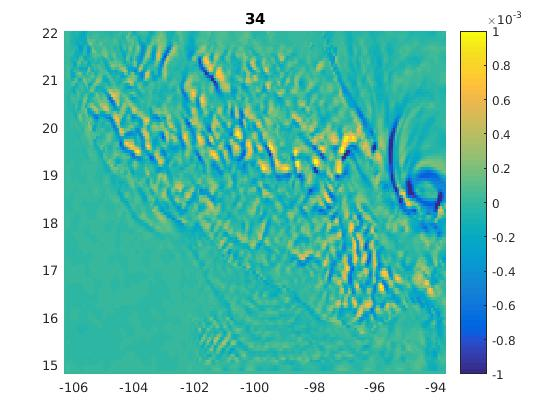
\includegraphics[width=0.35\textwidth]{div3}
  }\hfill
  \subfloat[ii=39]{%\label{fig:}
  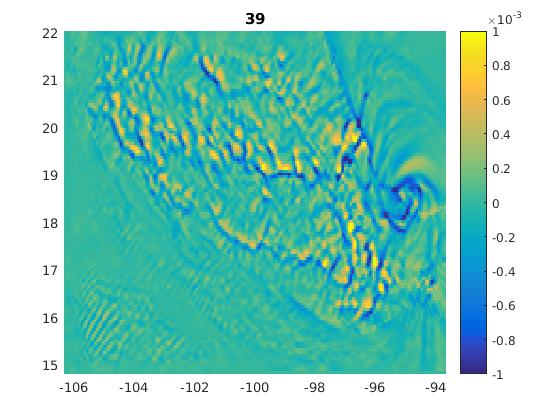
\includegraphics[width=0.35\textwidth]{div4}
  }\hfill
  \caption{Divergencia en 4 tiempos distintos, una divergencia positiva implica una fuente y una negativa indica hundimiento o sumidero.}%
\label{fig:dos}
\end{figure}
%%%%%